\documentclass[11pt]{book}
\usepackage{basecommon}
\usepackage[margin=1.5in, top=1in, headheight=14pt]{geometry}
\usepackage[backend=bibtex, natbib=true, autocite=superscript, style=authoryear-ibid]{biblatex}
\usepackage{hyperref}
\usepackage{url}
\usepackage{lineno}
\usepackage{graphicx}
\usepackage{fancyhdr}
\usepackage{tikz}
\renewcommand{\familydefault}{ptm} % try phv, ptm, ppl
\usetikzlibrary{positioning}
\usetikzlibrary{matrix}
\tikzset{
  treenode/.style = {shape=rectangle, rounded corners,
                     draw, align=center,
                     top color=white, bottom color=blue!20},
  root/.style     = {treenode, font=\Large, bottom color=red!30},
  env/.style      = {treenode},
  result/.style	={treenode, font=\Large, top color=blue!20, bottom color=blue!20}
}
\usepackage{pdfpages} % for inserting pdf pages
\addbibresource{../ch1/citations_annotated.bib}
\usepackage{setspace}
\doublespacing
\begin{document}
\pagestyle{fancy}
\fancyhf{}
\fancyhead[R]{\thepage}

%%%%%%%%%%%%%
% CHAPTER 3
%%%%%%%%%%%%%

\chapter{A Neural approach to harmonic analysis and prediction}

\section{Introducing Neural Networks}

I will now shift focus to supervised learning of the chorales using both non-recurrent and recurrent neural models, seeking to improve upon the baseline models presented in Chapter 2. Neural networks are able to engage in sophisticated decision-making by passing the input forward through the network and making more complex and abstract decisions in the hidden perceptron layers. As demonstrated in the literature review at the beginning of Chapter 2, neural networks are popular in computational musicology for their ability to perform highly complex pattern recognition over large datasets and generalize when given unexpected musical sequences. In particular, recurrent neural networks (RNNs) show great promise in sequence labelling because of their ability to incorporate contextual information about previous computations. In the case of next-step harmonic prediction, we discuss in Chapter 1 the constraints placed on the next harmony by the preceding harmonies. A satisfying harmonic sequence is additionally constrained by the ultimate goal of reaching resolution, and each harmony in the sequence can be labeled as a step towards or away from that goal. Therefore, I hypothesize that a next-step prediction model will benefit from additional features that denote the harmony chosen at the previous time step. This hypothesis will be evaluated by use of an "Oracle experiment."

\section{Methods}

\subsection{Two approaches to harmonization}

The experiments described in this chapter explore harmonization via two different methods. The first approach is predicting harmonization as a series of individual subtasks - identical to the approach in Chapter 2. Collection, a set of the predictions for all subtasks describe the harmony and its voicing for a given time step. The prediction of each subtask, moreover, is independent of the predictions for other subtasks at the same time step. Note that this does not particularly reflect the compositional process of a musician. The choice of inversion in Roman numeral analysis, for example, is dependent upon the chosen Roman numeral, and the selection of pitches for inner voices is dependent on the general harmony intended for that time step. The second approach groups a full set of predictions for all subtasks as a single prediction. This is referred to as the \textit{full harmonization} task, since the harmony and its voicing is decided by a single prediction. The set of output classes consists of all full sets of predictions observed in the training data, where each set of predictions is mapped to a single class, which describes a complete "harmonization". A single harmonization class might represent the following, for instance: D chord, major triad, root position, the 3rd above D in the alto, the 5th above in the tenor. This new approach adds a weak dependency between the subtasks because they are predicted collectively rather than separately. \\

In the full harmonization approach, approximately 5\% of harmonization classes in the test set do not occur in the training set. While this 5\% of classes represents a relatively infrequent set of harmonizations, the neural models will never predict these classes when evaluating test data. To understand why, imagine a model that accepts an image and classifies the content of the image as either a cat, a dog, or a bird. If the model is only shown cats and dog during training time, then it will update its parameters to reflect these observations - namely, that the input image is never of a bird but only either a cat or a dog. Consequently, an image of a bird in the test set will inevitably be misclassified. The images of bird are analogous to these infrequent harmonizations, which will essentially never be predicted. While we do not believe this classification discrepancy significantly affects the results achieved with the full harmonization approach, a better method for encoding harmony in future studies could eliminate this. 

\subsection{Oracle experiment}

Before incorporating recurrent models, I wanted to know if having the context of previous harmonies would in fact improve the model's ability to predict subsequent harmonies. In the field of natural language processing, an Oracle experiment refers to the inclusion to the addition of an "Oracle" in the data that always provides accurate information about some feature. By comparing the original model with the enhanced model, one can directly attribute the difference in error to the absence of the Oracle data. We use this experiment for the full harmonization task by including the correct harmonization class for the previous time step in each input vector. An improvement in performance with the Oracle data suggests that the harmonic information is a valuable component of the input data, and therefore favor a recurrent model that receives feedback for its computations at previous time steps. \\

Attributes 11 and 12 of the feature vector described in section 2.4.2 describe predictions for the harmonic analysis subtasks at the previous time step. Once GCT encoding was introduced, this became 3 features that described the root, base, and inversion of the previous harmony. By providing these features in the input vector, we simulate the feedback provided in a recurrent model from the computation at the previous time step. The baseline models and the "vanilla" neural network were re-evaluated using the Oracle features, using the same training-test split as before.

\subsection{Architecture for neural models}

All neural models were implemented in Torch, using the \texttt{rnn} module for the recurrent components. The "vanilla" neural network (NN) contained 3 layers, with one layer of varying sizes that was optimized based on performance over a validation set. The validation set consisted of 33 chorales randomly extracted from the training set. A lookup table was added as a layer of convolution that takes the input as a vector of indexed features and outputs a matrix where each column represents an embedding for a feature in the original input. After passing through the hidden layer, the intermediate output is transformed by a softmax to output a probability distribution over all possible output classes. The criterion used was negative log likelihood (NLL), and the objective is to continue training until NLL converges to a local minimum. All neural models were trained using backpropagation across all time steps of the chorale. Each chorale was padded with padding inputs mapped to a padding class in order to make each chorale a sequence a length equal to the length of the longest chorale. Optimal learning rates, based on performance over the validation set, varied from 0.01 to 0.001. \\

After noting the success of the Oracle experiment, two recurrent models were constructed with the objective of improving accuracy by feeding in the chorales as a \textit{sequence} of inputs. As discussed in Chapter 1, RNNs include recurrent connections that allow for feedback from the computation that occured at the previous time step. During the forward pass, at each time step in the data sequence, the RNN input layer receives an external input from the $i$th sequence $x^{(i)}_t$ as well as internal feedback from the hidden layer $h_{t}$, and then outputs a distribution $x_{t+1}$ for the next time step. Here, each element of the sequence is a feature vector describing a single melody note, drawn from the same dataset used for previous models. Internally, the network stores $h_t$ as a "memory" of the melody features at time $t + 1$, which will be used to predict the harmonization $x_{t+2}$, and so forth.

\begin{center}
\begin{tikzpicture}
  \matrix (m) [matrix of math nodes,row sep=3em,column sep=4em,minimum width=2em]
  {
     time \to & h_t & \to\\ 
     x^{(i)}_t & R & h_{t+1}\\
     \to & h_{t+1} \text{ (feedback)} & \to\\};
  \path[-stealth]
    (m-1-2) edge (m-2-2)
    (m-2-1.east|-m-2-2) edge [double] (m-2-2)
    (m-2-2.east|-m-2-3) edge [double] (m-2-3)
    (m-2-2) edge (m-3-2);
\end{tikzpicture}
\end{center}

The recurrent layer ($R$) accepts as input a sequence of input vectors describing each time step of a chorale and outputs a corresponding sequence of distributions describing the probability of each harmonization class at each time step. The most likely harmonization for each time step is selected by taking the $\argmax$ of that time step's output distribution, $h_{t+1}$.

$$\argmax h_{t+1} = \argmax_k
\begin{bmatrix} h_{{t+1}_1} \\ h_{{t+1}_2} \\ \vdots \\ h_{{t+1}_k}
 \end{bmatrix}
 $$

The first model is a "simple" recurrent neural network, or S-RNN \citep[p.~56]{goldberg2015nnlp}. The network has a single recurrent hidden layer, The second model is a 5-layer LSTM network with standard input, output, and forget gates. For both models, the hidden layers have a consistent size of 200 neurons. For regularization on the NN and LSTM model, we implemented dropout with probability 0.5 between all hidden-to-hidden layers. Dropout is a technique that address the overfitting problem associated with neural networks by "dropping" a random subset of activations in a given layer of the network. By eliminating a fraction of the signals at each layer, the network becomes comparable to a series of smaller, separately trained networks who outputs are averaged together to obtain a collective prediction.

\section{Results}

First, the "vanilla" neural network (NN) was evaluated on the same individual subtasks used in Chapter 2 for the baseline models, using GCT encoding. Table 3.1 provides the results for the NN performance on each subtasks for both training and test data. The training accuracy and NLL suggest that the neural model did not overfit on the subtasks. And comparing these results to the baseline model results shown in Figure 2.3, the neural network performs on average at the same accuracy rate as Random Forest, the strongest baseline model.

\begin{table}[h]
\begin{center}
\caption[Table caption text]{\textbf{"Vanilla" neural network accuracy.}}
\begin{tabular}{l *{5}{c}}
Task & Training NLL & Acc\% & Test NLL & Acc\% & Test MCCF \\ \hline
Root & 0.768 & 71.92\% & 1.164 & 58.66\% & 27.7\% \\
Base & 1.265 & 62.48\% & 1.694 & 55.09\% & 48.4\% \\
Inversion & 0.701 & 70.78\% & 0.770 & 67.86\% & 64.5\% \\
Alto & 0.903 & 67.90\% & 1.680 & 42.32\% & 21.7\% \\
Tenor & 0.900 & 67.57\% & 1.721 & 42.66\% & 20.7\%
\end{tabular}
\end{center}
\end{table}

The Oracle experiment demonstrated favorable results and improved performances across the board by a few percentages the board. Interestingly, the neural network performs only slightly better than logistic regression on harmonic analysis subtasks, but performs an average of 12.5\% better on prediction of inner voices. \\

\begin{table}[h]
\begin{center}
\caption[Table caption text]{\textbf{Baseline and neural model test accuracy, Oracle experiment. }}
\begin{tabular}{l *{5}{c}}
Classifier & Root & Base & Inversion & Alto & Tenor \\ \hline
Multi-Class Logistic & 59.75\% & 56.49\% & 64.43\% & 38.99\% & 38.93\% \\
Multinomial Na{\"i}ve Bayes & 54.31\% & 48.48\% & 63.06\% & 37.08\% & 34.10\% \\
Random Forests & 71.62\% & 65.85\% & 74.56\% & 53.91\% & 52.20\% \\ \hline
"Vanilla" Network (NN) & 60.86\% & 57.83\% & 69.67\% & 56.27\% & 46.67\%
\end{tabular}
\end{center}
\end{table}

Based on the favorable results from the Oracle experiment, the two recurrent models were constructed and evaluated. Na{\"i}ve Bayes was left out because it consistently underperformed in comparison to the other neural and non-neural models. The recurrent models took significantly longer to training, averaging between 18-24 hours. Random Forest, in contrast, only took 2-3 minutes to reach convergence. 

\begin{table}[h]
\begin{center}
\caption[Table caption text]{\textbf{Neural and baseline model accuracy, full harmonization task}}
\begin{tabular}{l c c c }
Model & Train NLL & Train & Test \\ \hline
Multinomial Logistic & -- & 42.74\% & 25.15\% \\
Random Forest & -- & 88.41\% & 30.38\% \\ \hline
NN & 1.127 & 67.41\% & 25.59\% \\
S-RNN & 0.756 & 45.95\% & 24.73\% \\
LSTM & 0.807 & 38.01\% & 29.35\%
\end{tabular}
\end{center}
\end{table}

Given that the MFFC frequency is 5\%, these results show a significant increase in accuracy over previous results. Although surprisingly, the recurrent models did not outperform the Random Forest model.


%%%%%%%%%%

\section{Discussion}

\subsection{Neural network results}

Neural networks proved capable learners for both harmonic analysis and prediction tasks. They outperformed the majority of baseline models and more than doubled accuracy when compared to the MCCF baselines for subtasks with more even class distributions (i.e. lower MCCF), such as the root and the alto and tenor voices. As discussed in Chapter 2, the uneven distribution of output classes means that the model's parameters will be updated predominantly to reflect the most frequent harmonization classes at the expense of learning to recognize rarer classes. This appears to be the case of the base and inversion tasks, where the network struggled to outperform the fairly accurate MCCF model. However, the overall performance of the network is strong considering the complexity of these musical tasks. \\

With respect to the recurrent neural models, it was surprising to see them outperform the Random Forest baseline model. This may be due to a variety of reasons, including a structural issue in the data or a class imbalance. Viewed another way, the Random Forest model performed exceedingly well considering that it does not receive the temporal feedback built into the recurrent models. We hypothesize that the Random Forest model likely generalized well despite the high frequency of a small set of harmonizations - a set mostly consisting of various tonic and dominant triad voicings. The non-recurrent models also benefitted greatly from the context already present in the input feature vector, which informs of the model of the position of the harmony within the measure and within the phrase. Hopefully, more work is done to examine the ability of both the Random Forest model and LSTM networks to perform other predictive musical tasks.

\subsection{Analyzing Random Forest harmonizations}

Figures 3.1 and 3.2 compare Bach's harmonizations against predicted harmonizations generated by the Random Forest model for the full harmonization task. The accuracy rating refers to the average accuracy of harmonization class prediction, where each class describes a full set of predictions for all subtasks. While the accuracy over test chorales varied greatly, two chorales were chosen to demonstrate the Random Forest harmonizations in both major and minor with accuracy levels close to the mean. The diagrams were created by reversing the feature extraction process by lookup feature indices and converting them back into musical terms. The scores were generated using a script that relied heavily on \textsc{music21}. Minor manual correction was then required to adjust the ranges of inner voices to the proper octave. Note that the "Original" score represents the Bach's score after the quantization process (Section 2.5). \\

These figures are clear evidence of the success of this model. The example harmonizations indicate a diversity of harmonic choices and voice-leading patterns. Most cadences are well-executed and provide a satisfying resolution to either tonic or dominant harmonies. In \textit{Helft mir Gotts G{\"u}te preisen} (Figure 3.1), two cadences in particular deserve note. Measure 12 features an authentic cadence to G major ($\flat$\rom{7}), despite no prior introduction of an F$\sharp$ in the soprano voice or other indication of this tonicization. The final measure, moreover, is correctly predicted as a Picardy cadence, resolving to an A major harmony in an A minor key. \\

The ends of phrases were also correctly identified, and the model typically output the same harmony for multiple beats when a fermata was being held. Examining other chorales, the model appears to struggle with more advanced harmonic progressions, particularly where tonicizations occur based on a tonic that is non-diatonic within the original key.
\clearpage

\fancyhf{}
\fancyhead[C]{\bfseries Figure 3.1}
\fancyhead[R]{\thepage}
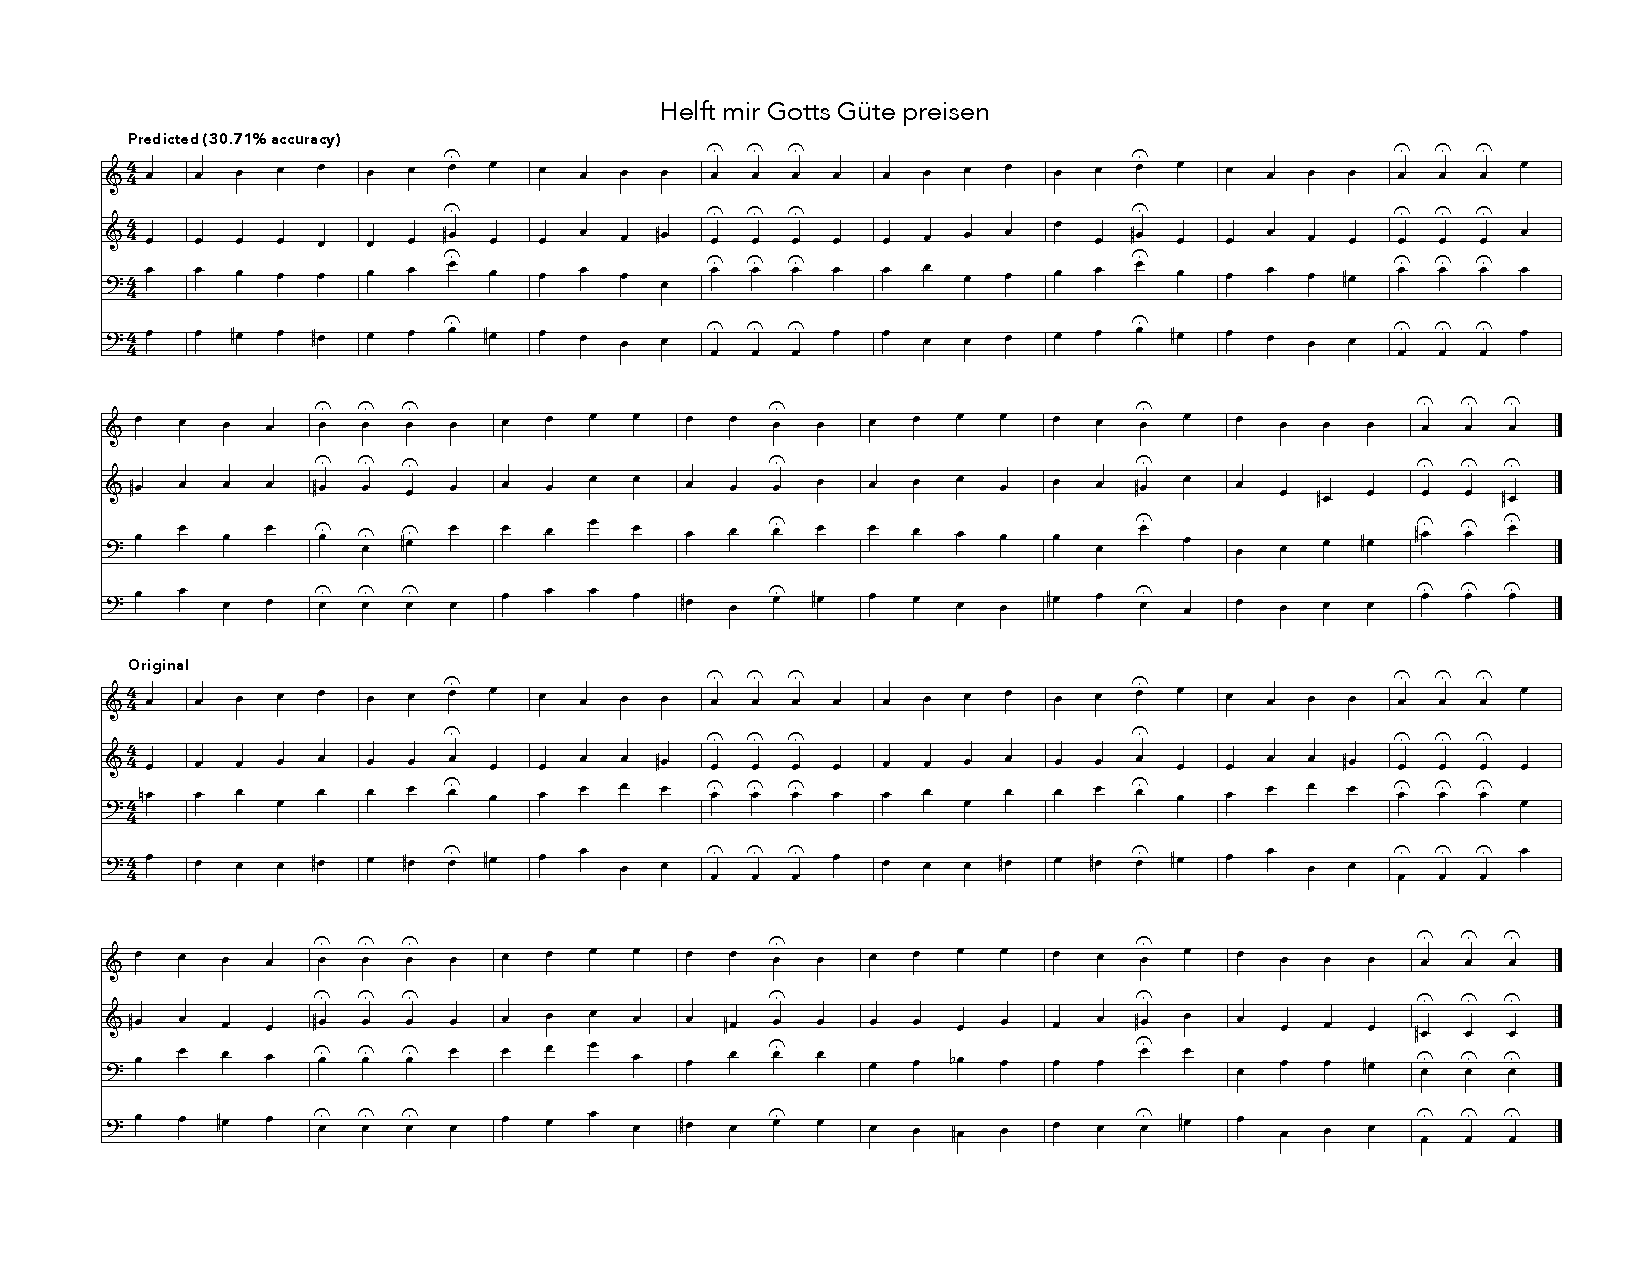
\includepdf[pages={1},pagecommand={\pagestyle{fancy}}]{examples/ex_minor_1.pdf}
\fancyhf{}
\fancyhead[C]{\bfseries Figure 3.2}
\fancyhead[R]{\thepage}
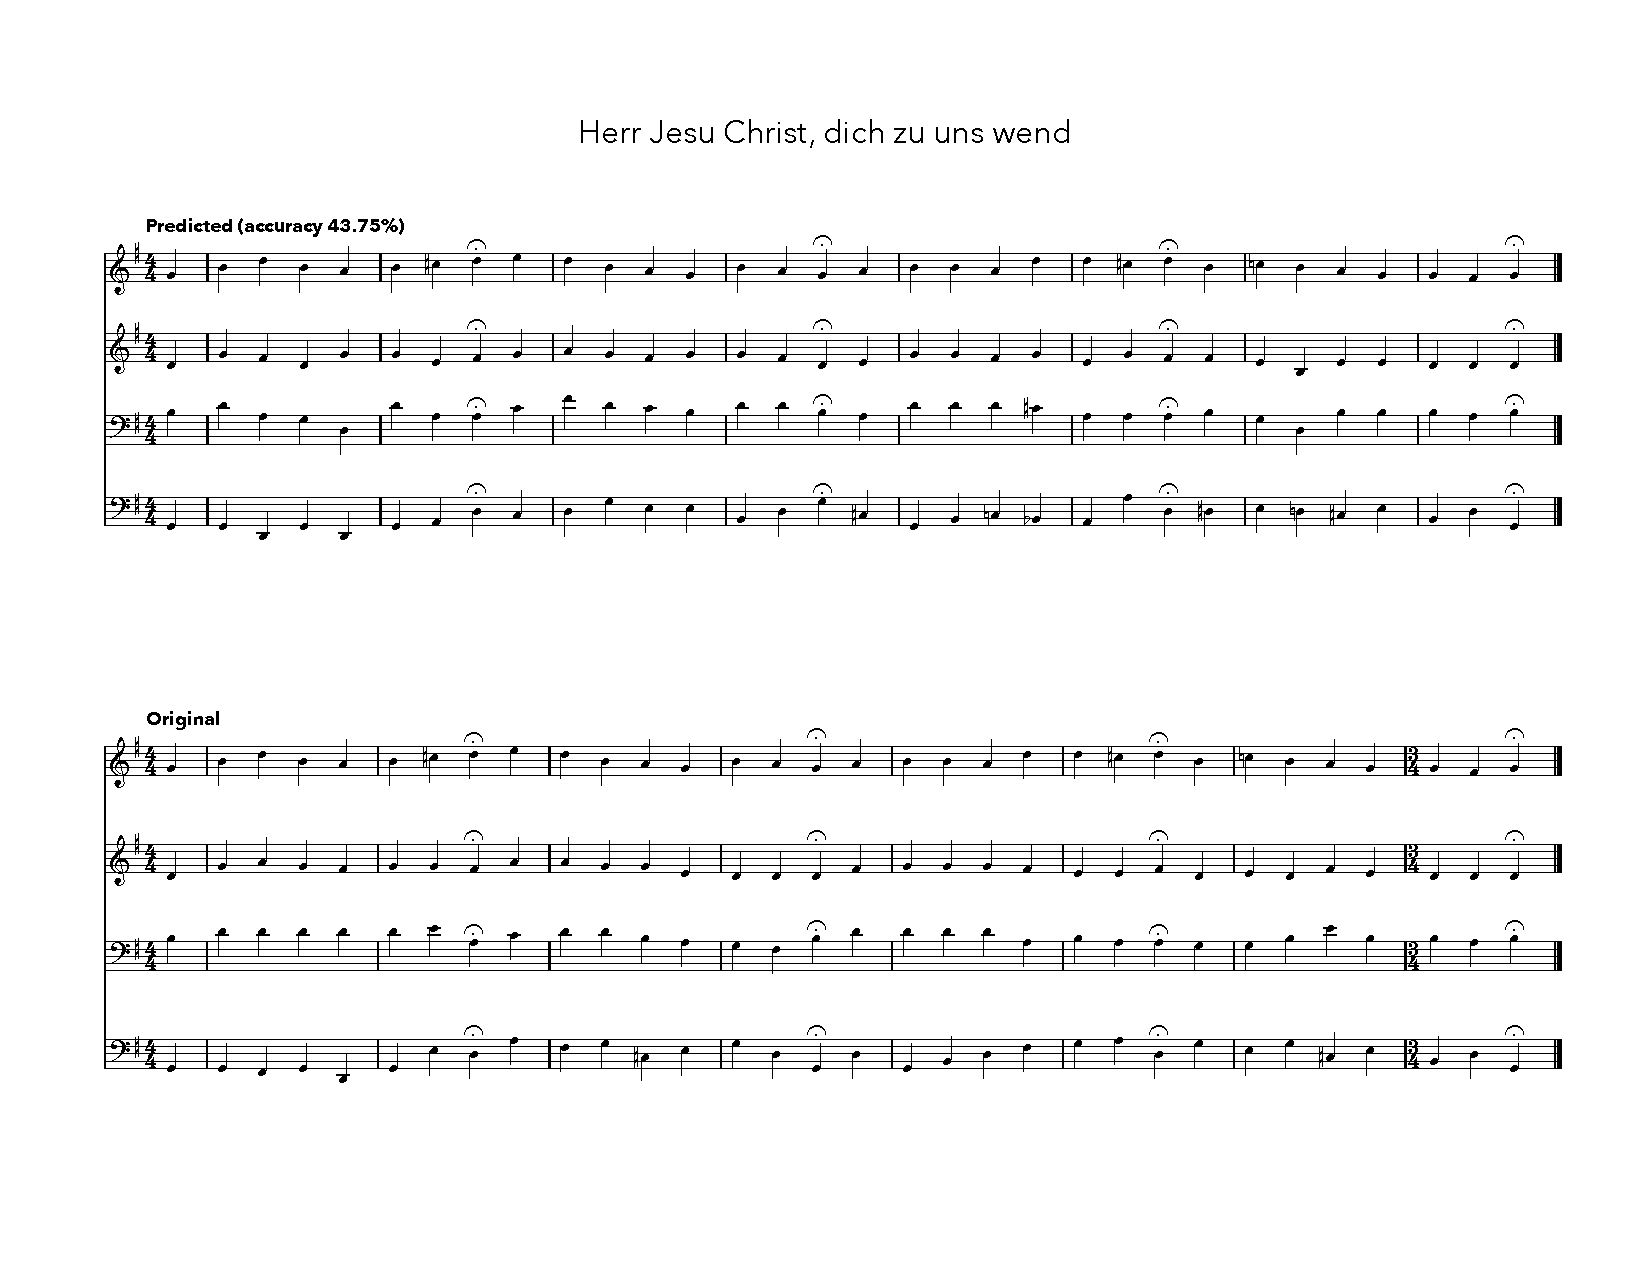
\includepdf[pages={1}, pagecommand={\pagestyle{fancy}}]{examples/ex_major_1.pdf}

\fancyhf{}
\fancyhead[R]{\thepage}

\subsection{Methods for an improved sequential subtask model}

Recall that the full harmonization task combines an independent series of subtasks into a single prediction task, where each harmonization class represents a set of predictions for the subtasks which are weakly interdependent. There are two significant flaws to this approach. First, the accuracy metric here is harsh because by combining a series of decisions into a single class, a much more fine-grained decision must be made to choose the correct class. This concern could be resolved by creating a more sophisticated accuracy metric that took into account its overall accuracy across all subtasks. The metric should weigh each subtask differently in order to reflect the different levels of musical importance associated with these harmonic aspects. The inversion, for example, is a much less decisive aspect of the harmony than the root or base. The selection of inner voices should also be weighed appropriately to reflect its role as expressing the harmony rather than deciding it. The alto and tenor voices can be often be assigned several different pairs of pitches that express the chosen harmony in a satisfying way. The second issue is that neither approach discussed in Section 3.2 recognizes the highly dependent nature of the subtasks. A \textit{sequential} subtask model may likely improve the results by recognizing the sequential nature of the tasks performed when harmonizing chorales. In particular, predictions for harmonic analysis subtasks would seem a highly useful source of information for predicting the inner voices. The choice of harmony constrains the possibilities of the inner voices since they must support that harmony. So while the current model only provides the melody-focused feature vector for each subtask, a stronger model will consider predictions made for previous subtasks at the same time step. Figure 3.3 shows the proposed ordering of those subtasks.

\begin{figure}[h]
\begin{center}
\caption{\textbf{Proposed model - sequential prediction of harmonization subtasks.}}
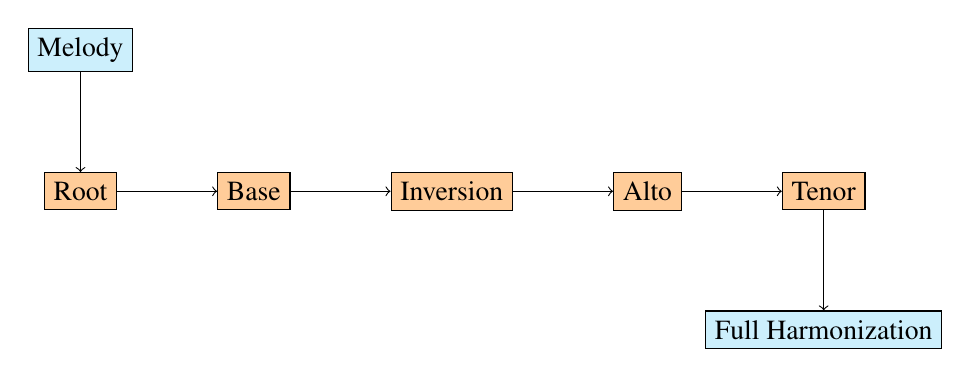
\begin{tikzpicture}
  [
    grow                    = down,
    sibling distance        = 6em,
    level distance          = 4em,
    edge from parent/.style = {latex-latexnew, line width=2pt, arrowhead=4cm}
  ]
  \begin{scope}[end/.style={rectangle,draw,fill=cyan!20},
  			env/.style={rectangle,draw,fill=orange!40}, node distance=1in]
  \node [end] (mel) {Melody};
  \node [env] (a) [below=0.5in of mel] {Root};
  \node [env] (b) [right=0.5in of a] {Base};
  \node [env] (c) [right=0.5in of b]{Inversion};
  \node [env] (d) [right=0.5in of c] {Alto};
  \node [env] (e) [right=0.5in of d] {Tenor};
  \node [end] (f) [below=0.5in of e] {Full Harmonization};
  \path[->] (mel) edge node {} (a);
  \path[->] (a) edge node {} (b);
  \path[->] (b) edge node {} (c);
  \path[->] (c) edge node {} (d);
  \path[->] (d) edge node {} (e);
  \path[->] (e) edge node {} (f);
  \end{scope}
\end{tikzpicture}
\end{center}
\end{figure}

We briefly describe this approach mathematically. Assume for the sake of notation that there are only three subtasks. Then the objective is to select
$$\argmax_{x, y, z} P(X=x, Y=y, Z=z | \boldX)$$ 

where X, Y, and Z are random variables associated with a specific subtask and can only takes value representing the subtask's output classes. $\boldX$ represents the input data, and let $\hat{x}, \hat{y}, \hat{z}$ be the predicted classes for the 3 subtasks. Then by the chain rule, we can show that
\begin{align}
\hat{x}, \hat{y}, \hat{z} &= \argmax_{x, y, z} P(X=x, Y=y, Z=z | \boldX) \\
				  &= \argmax_{x,y,z} P(X=x | \boldX, Y=y, Z=z) \cdot P(Y=y | \boldX, Z=z) \cdot P(Z=z | \boldX)
\end{align}

While mathematically equivalent, the implementation suggested by 3.2 would consist of separate classifiers for each subtask, where each classifier is trained to predict its respective subtask given the original input vector $\boldx$ along with the predictions for the previous subtasks in the sequence. To reduce the output space represented by all possible set of predictions for all subtasks, the model would only consider sets of predictions that occur in the training set.




%%%%%%%%%%%%
% CHAPTER 4
%%%%%%%%%%%%


\chapter{Chapter 4 - Looking forward}

\section{Further Exploration: The Bach Inventions}

It must be admitted that a model trained to harmonize chorales has limited utility in modern times (although it might have made Bach's work as \textit{Kapellmeister} a bit easier). Musicians only look to Bach's Chorales as early model compositions for 4 voices and for theory-related exercises. Moreover, the Chorales themselves use a limited rhythmic and textural vocabulary, since the rate of harmonic change and many other stylistic properties remain constant. This simplicity makes the chorales advantageous for statistical learning and allows our models to output a uniform set of harmonizations over all inputs. But as chorale harmonization is increasingly well-understood as a computational task, it is worth recognizing the ways in which the chorale harmonization model can be extended to more common musical processes. As one potential application, I will explore the task of composing a counterpoint line given an input melody, and how this might be approached from a computational standpoint. We will this task \textit{contrapuntal melodic generation}. This task is intentionally open-ended and could be applied to a wide variety of musical corpora. For this chapter, I will focus on how one might potentially implement such a model for Bach's 15 Inventions. Bach's Inventions were selected because they represent exemplary two-voice counterpoint compositions while also using Bach's harmonic language, which allows for comparison with the chorale model. Despite being written explicitly as musical exercises, the Inventions are far more melodically and rhythmically complex than the Chorales.

\subsubsection{Added complexity}
Generating harmonizations for inventions introduces several new layers of musical complexity that were not considered when harmonizing the chorales. One is \textit{rhythmic} complexity, since Invention melodies cannot be effectively quantized into uniform samples as we did with the Chorales, so a method for representing rhythmic features in the contrapuntal melody is need. One method for describing rhythm is to generate predictions at the level of the smallest rhythmic unit in the Invention. For example, if the smallest rhythmic unit in is the 32nd note, then each measure would be divided into 32 samples. A prediction of the pitch of the melody note for each sample is then output, where the "pitch" can alternatively be a rest. Finally, the duration of each melody note or rest can be measured as the number of consecutive samples for which the same pitch or rest is predicted by the model. \citet{eck2002blues} found this approach effective for composing blues melodies. An similar but alternative method for describing pitch alongside rhythm was proposed by \citet{franklin2006jazz}, where separate LSTMs are trained to decide pitch and duration. \\

An additional layer of complexity to consider is the need for subject identification. In contrast to the Chorales, one or more melodic motives govern the development of the entire work, and each motive is restated in various transformations. Collectively, we refer to these motives, or subjects, as the "invention" of the work \citep[p.~10]{dreyfus1996bach}. Dreyfus argues that the composition process behind an Invention is in many ways analogous to process behind writing an oration, which he describes in terms of Ciceronian rhetoric. This comparison is meant to emphasize Bach's "obsession with inventive process" \citep[p.~35]{dreyfus1996bach}. In order to model the inventive process, identifying of the subject is critical to interpreting the initial stage of musical creating behind the work - labelled as \textit{invention}, the first stage of rhetoric. The "invention" of the work reveals the melodic, harmonic, and rhythmic material used in the Invention, and features from the subject should be extracted to create contrapuntal melodies. \\

A final layer of complexity to note is the \textit{form}, or large-scale structure of the Invention. Inventions typically consist of a series of thematic statements interleaved with episodes - modulatory sections that are melodically derived from the subject and create transitions between thematic statements in different keys. The remaining sections might be termed "elaborations", which include cadences at the ends of episodes and codettas that occasionally come at the end of an Invention. Each type of section has a specific set of conventions that govern its structure as well as the relationship between the two voices. Potential methods for addressing these complexities is described below.

\subsubsection{Subject identification}
Bach's Inventions are two-voice compositions, where the lower voice can be characterized as a \textit{function} of the upper voice. In order for the model to learn the harmonic and rhythmic material that Bach employs in the work, the model should first identify and extract features from the Invention's primary \textit{subject}. Identifying the subject generally straightforward for the listener, since the primary subject is typically the first statement in the upper voice. However, inventions can contain multiple subjects with varying levels of importance. And in Invention No. 6 in E major, Bach introduces two subjects of equal importance and develops them both consistently throughout. Therefore, a better approach might be to identify subjects by selecting melodic ideas based on the frequency with which they are restated. \citet{dreyfus1996bach} notes that the frequency of a subject is directly correlated with its importance in the Invention - a principle of repetition that is generally true of melodies in Western music. One candidate algorithm for subject identification based on repetition is hierarchal agglomerative clustering (HAC), which can learn to "cluster" melodic segments based on a supplied distance metric. \citet{nagler2014schubot} applied HAC to the task of motivic analysis in Schubert's song cycle \textit{Die Winterreise} and found promising results in extracting the main motive from each song. However, a significant difficulty in subject identification would be the harmonic and rhythmic transformations that are often applied to the subject when it is restated. For this task, it could be useful to encode the melody as a series of intervals rather than pitches in order to identify subjects in their original form as well as their transformed state. \\

\begin{figure*}[h]
\caption{ The subject and transformations in Invention No. 4 in D Minor, BWV 775.  }
\centerline{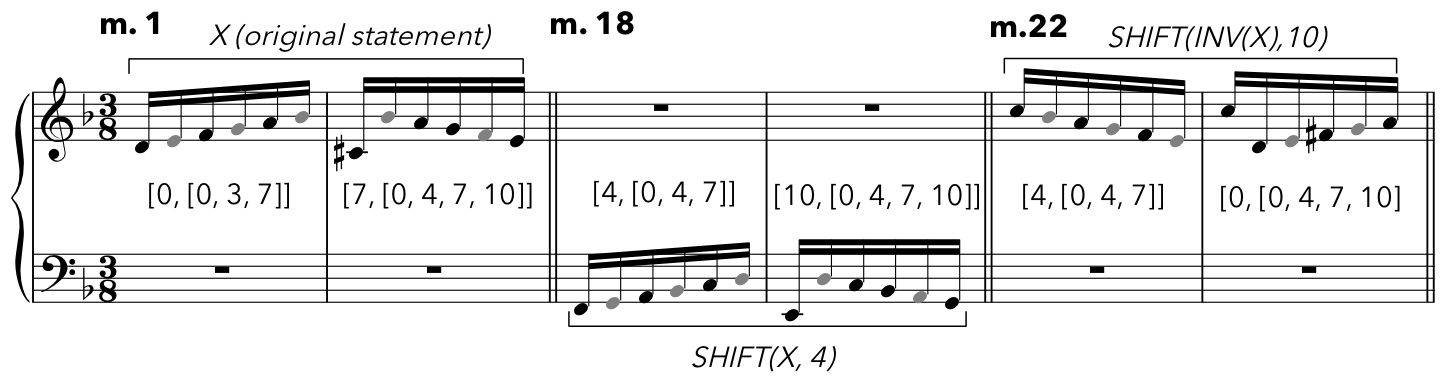
\includegraphics[scale=0.3]{examples/ex1}}
\end{figure*}


\subsubsection{Form identification}
Once rhythmic and melodic features are extracted from the most prominent subjects, the model can use these to analyze the large-scale structure of the Invention and divide the work into a series of sections. One classifier could be trained to create the general boundaries of each section, while a separate classifier could label each section as a thematic statement ($T$), episodes ($S$), and elaborations ($E$) by analyzing if and how the subject is presented in the upper voice. Complete, sequential statements of the subject suggest a thematic statement, while partial and transformed subject statements will suggest an episode. Elaborations will most likely differentiate themselves by the unique and less repetitiv e melodic material.

\subsubsection{Harmonic identification}
Before generating the melody, a useful preprocessing step would be to perform harmonic analysis over the upper voice. The classifier would be trained to accept the upper voice as input and output a sequence of corresponding harmonic encodings. This task is well-suited to the model presented in Chapter 2 and 3, where information about a segment of the melody would be classified as a GCT-encoded harmony. While many pleasant melodies can be generated for the counterpoint melody, the most crucial constraint is harmonic agreement. A crucial purpose of the contrapuntal lower voice is to support the upper voice in harmony. The upper voice typically guides the progression, while the lower voice may echo and reinforce harmonic transitions, as Figure 3a illustrates. \\

The primary technique for implying harmonies is the use of scalar and triadic passages. Not coincidentally, many of Bach's subjects are constructed to facilitate various transformations (\textit{SHIFT}, \textit{INV}, \textit{AUGMENT}, etc.) and be harmonically indicative. However, given a scalar or triadic passage, it can be difficult to determine which of many potential chords is most strongly implied. There are several important indicators, including the harmony in the previous melodic unit and the beat strength of the notes in the current unit. A recurrent model would likely perform well on this task because of the sequential format of the data (representing the upper voice as a \textit{sequence} of melodic units) and the feedback loop that would provide information about preceding harmonies. The size of each melodic unit, however, is an additional parameter that would require adjustment since the implied harmonies have varying durations (Figure 3b). \\

\begin{figure*}[h]
\caption{ Excerpts from Invention No. 13 in A Minor, BWV 784.  }
\centerline{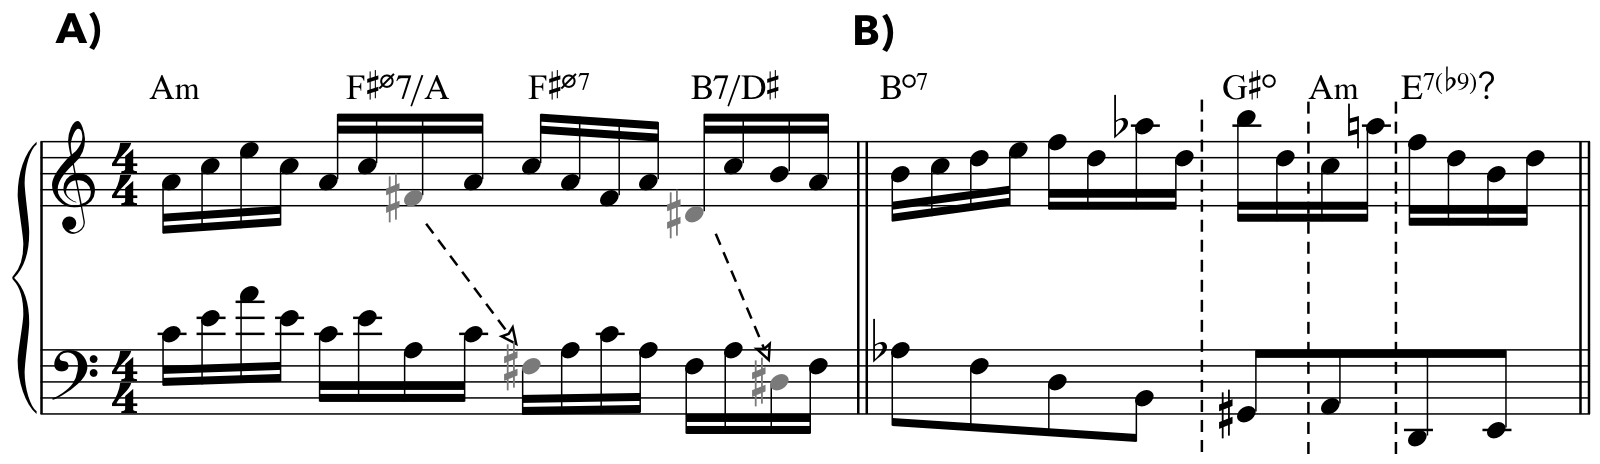
\includegraphics[scale=0.27]{examples/ex2}}
\end{figure*}

\subsubsection{Contrapuntal melodic generation}
Using the structural information gathered during preprocessing, a final classifier is trained to generate contrapuntal melodies. The classifier would accept input features describing the current relevant subject, the current section of the form, and the current implied harmony, as well as melodic features related to the upper voice near time $t$. The output feature would describe the most likely pitch for time $t$, with an implied duration of the length of the time step. Consecutive time steps of the same pitch could be merged to represented longer notes. \\
The generalization of this model allows for a wide range of corpora to be incorporated into the training data. Stylistically similar candidates include Bach's Sinfonias (the 3-voice equivalent of the Inventions) and the Fugues. Stylistically separate candidates include Palestrina's masses and motets, which feature significant contrapuntal composition and development of melodic motives in multiple voices. The larger dataset available for training will very likely improve model performance, in comparison to the computationally small dataset of chorales u0sed in this paper. Further work should be done to explore this extension of the harmonization task to various musical corpora.

\section{Conclusion}

In this paper, the objective was to apply a variety of neural and non-neural models to different musical processes involved in the task of chorale harmonization. These models are meant to supplement existing work on computational approaches to generative and completive musical tasks, not to replace human musical analysis or composition. The Random Forest model and recurrent neural models proved most effective in learning the various subtasks associated with harmonization, and in the future they should be evaluated on similar musical tasks, such as the generation of contrapuntal voices. The accuracy results from experiments with these computational models demonstrate a promising ability to learn musical structure and connect temporally distant events.

\subsection{Code and related files}

All code and data related to this paper is freely available on GitHub at\\ \url{https://github.com/glasperfan/thesis/}.

\newpage

\printbibliography

\end{document}